\documentclass[../Master.tex]{subfiles}

\begin{document}

\chapter{Experimental section}\label{cha:experimental-section}

\section{General information}
The reagents and solvents used in this thesis are commercially available and were generally used without further purification.

The THF used for the synthesis of the DikDiEst and DikDiCN has been anhydrified on sodium/benzophenone and distilled before use.

The synthesis of the DikDiCN and DikDiEst was carried out according to the synthesis methods reported in previous work. In particular, the synthesis conditions relating to DiCN are reported in the article \cite{carlucci_heterometallic_2010} and in Marco Visconti's thesis. The conditions relating to the synthesis of DikDiEst and DikDiAc are instead reported in the thesis "" by Simone Galeazzi.

\todo[inline]{Mi manca il titolo della tesi di Marco Visconti, inoltre il titolo della tesi di Simone in italiano on in inglese? Per quanto riguarda fornitore reagenti dovrebbe essere Merck?}

The reactions were carried out under aerobic conditions, except for the synthesis reaction of the
DikDiCN ligand and DikDiEst, were carried out under anhydrous conditions in a nitrogen atmosphere, as specified in the respective synthesis conditions.

The characterisation techniques used are FT-IR-ATR, NMR and UV; the instrumentation is given below:

\begin{itemize}
	\item Analytical scale: METTLER AE 200
	\item IR spectrophotometer: PerkinElmer Frontier TM FT-IR/FIR
	\item NMR spectrometer: Brucker NEO 400
	\item UV spectrophotometer:
	      \todo[inline]{manca nome UV, per gli spettri della parte della prof Mussini}
	\item Sonicator: Branson 5510 sonicator
	\item Centrifuge: Eppendorf 5430, 50 mL propylene tubes.
\end{itemize}
\section{DikDiEst}

\subsection{Synthesis}

\begin{center}
	\begin{tabular}[b]{lccccccc}
		\toprule
		Reagent                 & CAS       & MW  [\(g \ mol^{-1}\)] & m [g] & n [mmol] & SR   \\
		\midrule
		methyl 4-acetylbenzoate & 3609-53-8 & 178.19                 & 4.400 & 24.69    & 1.20 \\
		dimethyl terephthalate  & 120-61-6  & 194.19                 & 4.000 & 20.60    & 1.00 \\
		NaH, mineral dispersion & 7646-69-7 & 23.998                 & 1.132 & 47.17    & 2.30 \\
		\bottomrule
	\end{tabular}
\end{center}

The reaction is carried out under N$_{2}$ atmosphere, the reactants are carefully dried beforehand.\\
In a flask, 1.132 g of NaH dispersion in mineral oil are washed with anhydrous THF (15 mL x 2).\\
4.0 g of methyl 4-acetyl benzoate and 4.4 g of dimethyl terephthalate are dissolved in 45 mL of anhydrous THF, and then NaH suspension in THF is added with pasteur pipette.\\
The mixture is heated to reflux overnight. \\
Evaporation of the solvent under vacuum gives a dark brown compound. The solid is taken up in water and acidified with HCl 20\% in an ice bath. Taking care to leave it to react for a few hours and checking the pH to make sure it is acid. More water is added if mixing is particularly difficult.\\
The raw product is recovered as a yellow solid by filtration with a Buchner funnel.
To eliminate the impurities of the remaining reagents the solid is washed with chloroform and with diethyl ether. The solid is lastly collected on a Buchner funnel and dried. Yield: 92\%, 8.67 g of product.

\subsection{Characterization}
\subsubsection{NMR}
\begin{figure}[h!]
	\centering
	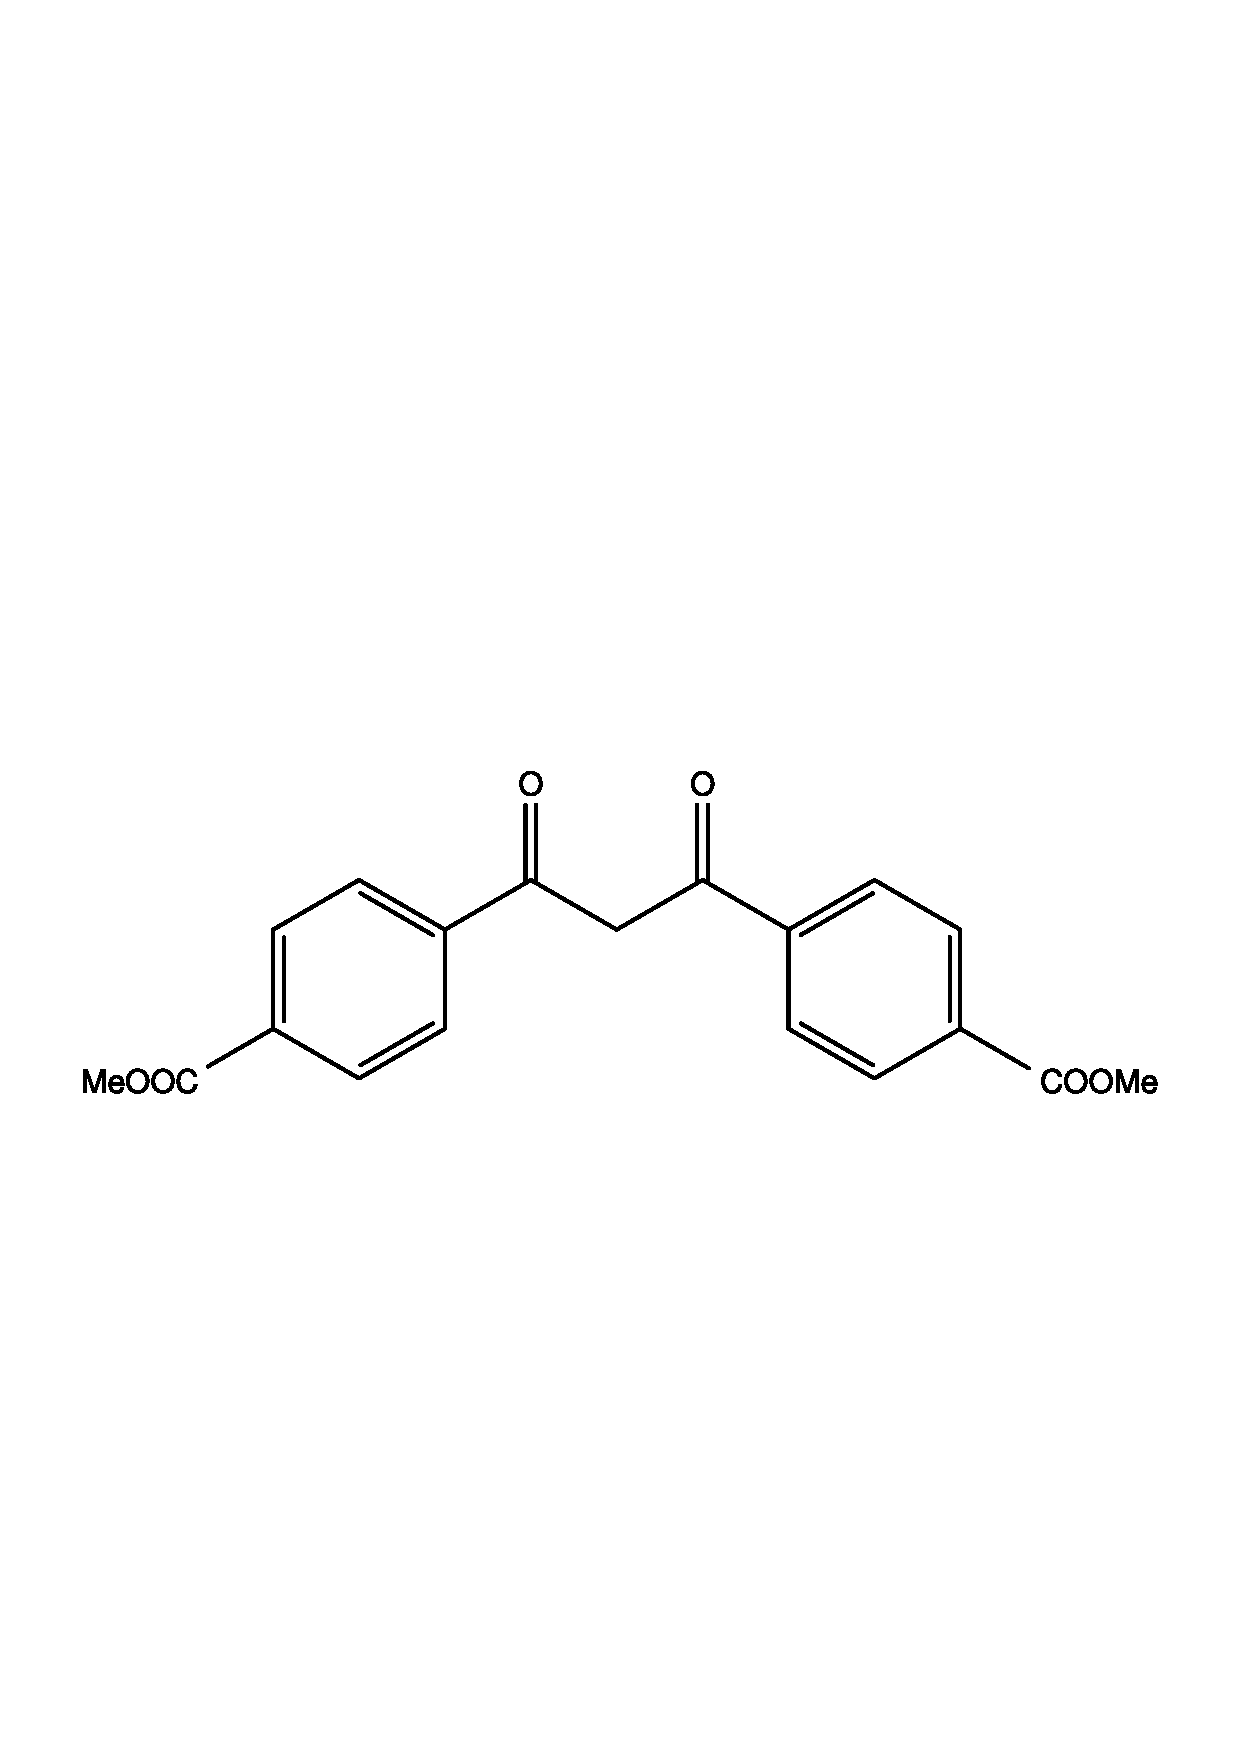
\includegraphics[width=12cm,keepaspectratio]{Spectra/nmr/dikest2.pdf}
	\caption{DikDiEst \NMR*{1,H}(400)[CDCl3]}
\end{figure}
\begin{figure}[h!]
	\centering
	\includegraphics[width=12cm,keepaspectratio]{Spectra/nmr/dikest.pdf}
	\caption{DikDiEst \NMR*{1,H}(400)[CDCl3], zoom on diagonistic peaks}
\end{figure}

\newpage
\section{DikDiAc}
\subsection{Synthesis}

\begin{center}
	\begin{tabular}[b]{lccccccc}
		\toprule
		Reagent  & CAS       & MW [\(g \ mol^{-1}\)] & m [g] & n [mmol] & SR \\
		\midrule
		DikDiEst & -         & 340.31                & 1.000 & 2.940    & 1  \\
		LiOH     & 1310-65-2 & 23.95                 & 1.411 & 58.80    & 20 \\
		\bottomrule
	\end{tabular}
\end{center}

In a small beaker, 1.411 g of freshly ground LiOH is dissolved in 10 mL of water. In an flask, 1.000 g of 4,4'-malonyldibenzoate is suspended in 10 mL of THF, then the LiOH solution is slowly added. The mixture is allowed to react 7 hours at room temperature under vigorous stirring. It is then proceeded by extracting with \(CHCl_{3}\) (3x25 mL). The aqueous phase is collected and acidified with 10 \% HCl to acidic pH, observing the formation of straw-yellow precipitate. The solid is recovered by filtration over buchner and allowed to air dry. Yield: 65\%

\newpage
\subsection{Characterization}
\subsubsection{NMR}
\begin{figure}[h!]
	\centering
	\includegraphics[width=12cm,keepaspectratio]{Spectra/nmr/dikdiac.pdf}
	\caption{DikDiAc \NMR*{1,H}(400)[DMSO-d6]}
\end{figure}
\begin{figure}[h!]
	\centering
	\includegraphics[width=12cm,keepaspectratio]{Spectra/nmr/dikdiac2.pdf}
	\caption{DikDiAc \NMR*{1,H}(400)[DMSO-d6], zoom on diagnostic peaks}
\end{figure}

\newpage
\subsubsection{IR}

\begin{figure}[h!]
	\centering
	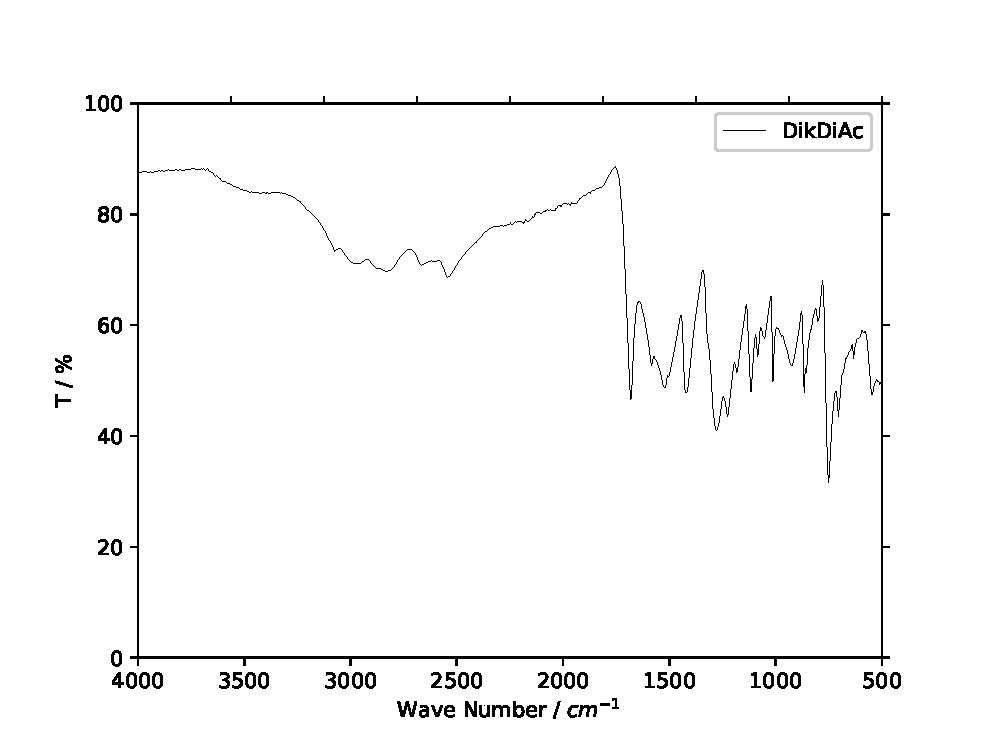
\includegraphics[width=12cm,keepaspectratio]{Spectra/ir/DikDiAc.eps}
	\caption{DikDiAc IR spectrum}
\end{figure}

\section{PyrDiEst}
\subsection{Synthesis from DikDiEst}
\subsubsection{EtOH}
\begin{center}
	\begin{tabular}[b]{lccccccc}
		\toprule
		Reagent                      & CAS      & MW \([g \ mol^{-1}]\) & V [mL] & m [g] & n [mmol] & SR  \\
		\midrule
		DikDiEst                     & -        & 324.332               & -      & 1.012 & 2.9      & 1   \\
		\(N_2H_4 \cdot H_2O \ 65\%\) & 302-01-2 & 50.05                 & 1.096  & 1.130 & 7.25     & 2.5 \\
		\bottomrule
	\end{tabular}
\end{center}
A typical synthesis is described here:
1.012 g of DikDiEst is suspended in 20 mL of EtOH in a 50 mL flask. The mixture is left in ultrasonic bath for 30'. 1.096 mL of hydrazine monohydrate 65\% water solution  are slowly added to the mixture that is then heated to reflux overnight.\\
The compound is collected as a pale yellow solid on a teflon funnel.
\newpage
\subsubsection{DMF}
\begin{center}
	\begin{tabular}[b]{lccccccc}
		\toprule
		Reagent               & CAS       & MW \([g \ mol^{-1}]\) & V [mL] & m [g] & n [mmol] & SR  \\
		\midrule
		DikDiEst              & -         & 324.332               & -      & 0.370 & 1.46     & 1   \\
		\(N_2H_4 \cdot H_2O\) & 7803-57-8 & 50.05                 & 0.356  & 0.370 & 3.65     & 2.5 \\
		\bottomrule
	\end{tabular}
\end{center}
A typical synthesis is described here:
0.370 g of DikDiEst is suspended in 15 mL of DMF in a 50 mL flask. The mixture is left in ultrasonic bath for 30'. 0.350 mL of hydrazine monohydrate are slowly added to the mixture that is then heated to 150°C overnight.\\
Evaporation of the solvent under vacuum gives a white ivory solid. The compound is then washed adding 25 mL of ethanol and heat to reflux for 2 hours. The solid is collected on a Buchner funnel.
\subsubsection{DMSO}
\begin{center}
	\begin{tabular}[b]{lccccccc}
		\toprule
		Reagent               & CAS       & MW \([g \ mol^{-1}]\) & V [mL] & m [g]  & n [mmol] & SR \\
		\midrule
		DikDiEst              & -         & 324.332               & -      & 0.5001 & 1.46     & 1  \\
		\(N_2H_4 \cdot H_2O\) & 7803-57-8 & 50.05                 & 0.356  & 0.37   & 7.39     & 5  \\
		\bottomrule
	\end{tabular}
\end{center}
A typical synthesis is described here:
0.500 g DikDiEst is solubilised in 20 mL DMSO in a 50 mL flask. The mixture is left in an ultrasonic bath for 30 min. 0.350 mL hydrazine monohydrate is slowly added to the mixture, which is then heated at 150°C overnight. The mixture is allowed to cool to RT and then diluted 1:20 with distilled water. The mixture is left to cool in the refrigerator and a fine white precipitate is observed to form. It is centrifuged to recover the product, which is finally recovered with EtOH. To avoid loss of product, crystallisation is carried out directly with subsequent filtration on buchner. The product is left to air dry.

\subsection{Synthesis from UnsDiEst}

\paragraph{Acetic acid}

\begin{center}
	\begin{tabular}[b]{lccccccc}
		\toprule
		Reagent               & CAS       & MW \([g \ mol^{-1}]\) & V [mL] & m [g] & n [mmol] & SR \\
		\midrule
		UnsDiEst              & -         & 324.332               & -      & 0.370 & 1.14     & 1  \\
		\(N_2H_4 \cdot H_2O\) & 7803-57-8 & 50.05                 & 0.171  & 0.166 & 3.42     & 3  \\
		\bottomrule
	\end{tabular}
\end{center}

A typical acetic acid reaction is conducted as follows.\\
This is done by dispersing 0.370 g of UnsDiEst in 8 mL of acetic acid, under strong agitation. 0.171 mL of hydrazine monohydrate is slowly added. The mixture is brought to reflux and left to react for 24h. The mixture is allowed to cool to room temperature and then refrigerated. Precipitation of white solid is observed, which is separated by filtration.

\newpage
\paragraph{EtOH with HCl}

\begin{center}
	\begin{tabular}[b]{lccccccc}
		\toprule
		Reagent               & CAS       & MW \([g \ mol^{-1}]\) & V [mL] & m [g] & n [mmol] & SR \\
		\midrule
		UnsDiEst              & -         & 324.332               & -      & 0.300 & 0.92     & 1  \\
		\(N_2H_4 \cdot H_2O\) & 7803-57-8 & 50.05                 & 0.134  & 0.138 & 2.76     & 3  \\
		\bottomrule
	\end{tabular}
\end{center}

A typical reaction with MeOH and HCl is conducted as follows.\\
0.300 g of UnsDiEst is dispersed in 5 mL of 20\% HCl solution in MeOH under vigorous stirring. 0.134 mL of hydrazine monohydrate is slowly added. The mixture is left stirring.

\paragraph{EtOH with pyridine}

\begin{center}
	\begin{tabular}[b]{lccccccc}
		\toprule
		Reagent               & CAS       & MW \([g \ mol^{-1}]\) & V [mL] & m [g] & n [mmol] & SR \\
		\midrule
		UnsDiEst              & -         & 324.332               & -      & 0.300 & 0.92     & 1  \\
		\(N_2H_4 \cdot H_2O\) & 7803-57-8 & 50.05                 & 0.134  & 0.138 & 2.76     & 3  \\
		\bottomrule
	\end{tabular}
\end{center}

A typical reaction with MeOH and pyridine is conducted as follows. \\
0.300 g of UnsDiEst is dispersed in 5 mL of 20\% pyridine solution in MeOH under vigorous stirring. 0.134 mL of hydrazine monohydrate is slowly added. The reaction mixture refluxes for 2 h, and is allowed to cool first at RT and then in the refrigerator. The precipitate formed is filtered over buchner and allowed to air dry.

\paragraph{EtOH}

\begin{center}
	\begin{tabular}[b]{lccccccc}
		\toprule
		Reagent               & CAS       & MW \([g \ mol^{-1}]\) & V [mL] & m [g] & n [mmol] & SR \\
		\midrule
		UnsDiEst              & -         & 324.332               & -      & 0.500 & 1.54     & 1  \\
		\(N_2H_4 \cdot H_2O\) & 7803-57-8 & 50.05                 & 0.222  & 0.231 & 4.62     & 3  \\
		\bottomrule
	\end{tabular}
\end{center}

A typical reaction with EtOH and pyridine is conducted as follows. \\
0.500 g of UnsDiEst is dispersed in 5 mL of EtOH under vigorous stirring. 0.222 mL of hydrazine monohydrate is slowly added. The reaction mixture refluxes for 5 h, and is allowed to cool first at RT and then in the refrigerator. The precipitate formed is filtered over buchner and allowed to air dry.

\newpage
\subsubsection{Characterization}
\newline
\paragraph{NMR}

\begin{figure}[h!]
	\centering
	\includegraphics[width=12cm,keepaspectratio]{Spectra/nmr/pyrest.pdf}
	\caption{PyrDiEst \NMR*{1,H}(400)[THF-d8]}
\end{figure}

\begin{figure}[h!]
	\centering
	\includegraphics[width=12cm,keepaspectratio]{Spectra/nmr/pyrest2.pdf}
	\caption{PyrDiEst \NMR*{1,H}(400)[THF-d8], zoom on diagonistic peaks}
\end{figure}
\newpage
\paragraph{IR}
\begin{figure}[h!]
	\centering
	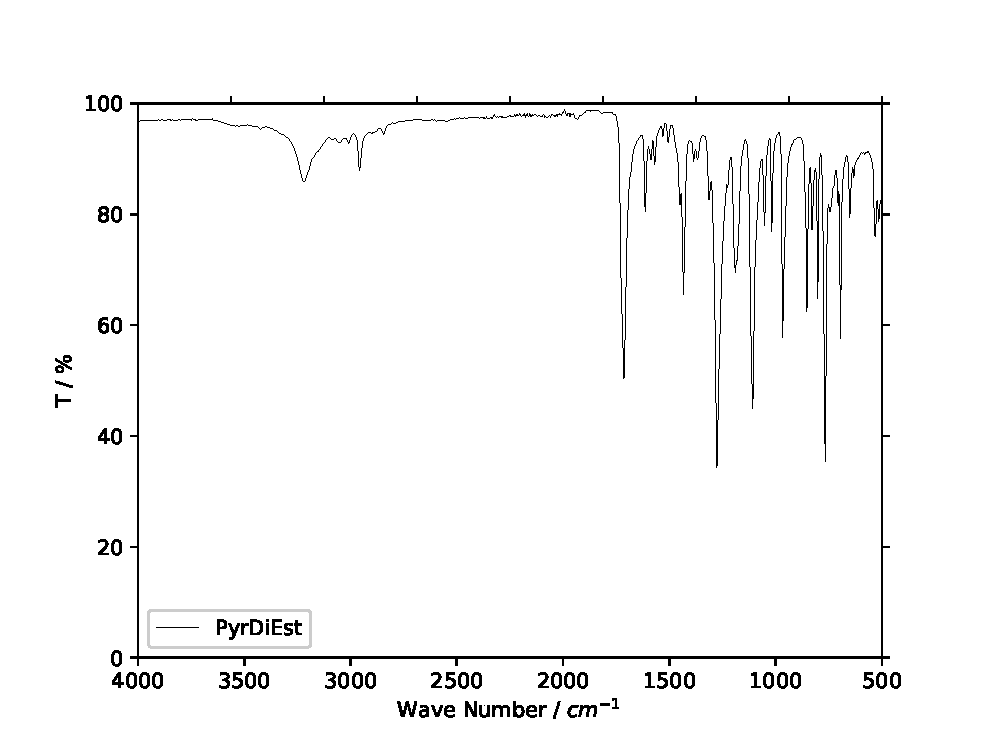
\includegraphics[width=12cm,keepaspectratio]{Spectra/ir/PyrDiEst.eps}
	\caption{PyrDiEst IR spectrum}
\end{figure}

\section{UnsDiEst}
\subsection{Synthesis}
\begin{center}
	\begin{tabular}[b]{cccccccc}
		\toprule
		Reagent                 & CAS       & MW \([g \ mol^{-1}]\) & m [g] & n [mmol] & SR  \\
		\midrule
		methyl 4‐formylbenzoate & 1571-08-0 & 178.18                & 0.500 & 2.8      & 1   \\
		methyl 4‐acetylbenzoate & 3609-53-8 & 164.16                & 0.550 & 3.5      & 1.2 \\
		NaOH                    & 1310-73-2 & 39.998                & 0.230 & 5.6      & 2   \\
		\bottomrule
	\end{tabular}
\end{center}

In a small beaker, 230 mg of freshly ground NaOH is dissolved in 10 mL of methanol. \\
In a flask, 500 mg methyl 4-formylbenzoate and 550 mg methyl 4-acetylbenzoate are dissolved in 5 mL MeOH. The mixture is placed under vigorous stirring in an ice bath. The freshly prepared sodium hydroxide solution is slowly added. The reaction is left to react overnight. \\
The yellowish solid is collected on Buchner funnel and allowed to air dry. Yield 94\%, 0.85 g of product.
\newpage
\subsection{Characterization}
\subsubsection{NMR}

\begin{figure}[h!]
	\centering
	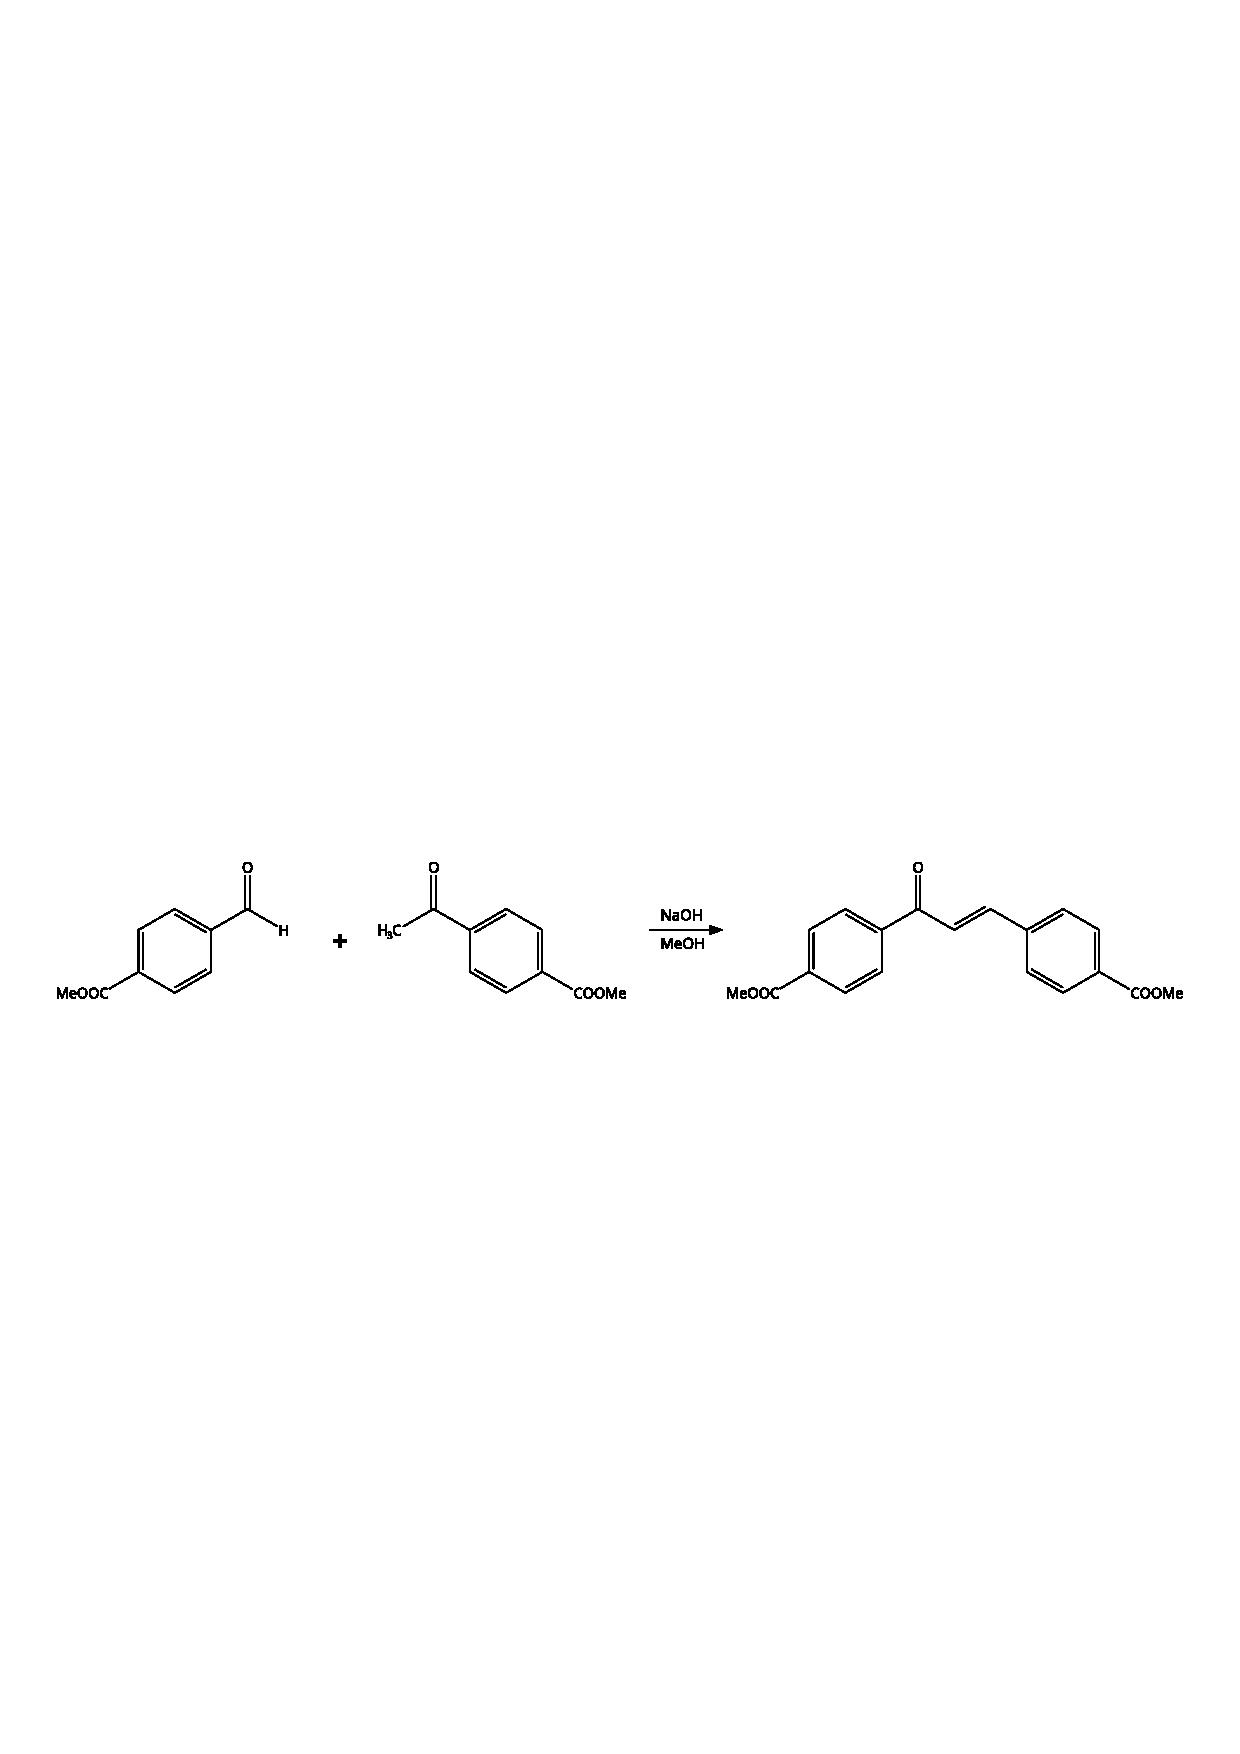
\includegraphics[width=12cm,keepaspectratio]{Spectra/nmr/aldolica.pdf}
	\caption{UnsDiEst \NMR*{1,H}(400)[CDCl3]}
\end{figure}

\begin{figure}[h!]
	\centering
	\includegraphics[width=12cm,keepaspectratio]{Spectra/nmr/aldolica2.pdf}
	\caption{UnsDiEst \NMR*{1,H}(400)[CDCl3], zoom on diagonistic peaks}
\end{figure}

\newpage \section{PyrDiAc}
\subsection{Synthesis}
\begin{center}
	\begin{tabular}[b]{lccccccc}
		\toprule
		Reagent  & CAS       & MW \([g \ mol^{-1}]\) & m [g]  & n [mmol] & SR \\
		\midrule
		PyrDiEst & -         & 336.47                & 0.3023 & 0.8988   & 1  \\
		LiOH     & 1310-65-2 & 23.95                 & 0.4505 & 17.796   & 20 \\
		\bottomrule
	\end{tabular}
\end{center}

In a small beaker, 0.4505 g of freshly ground LiOH is dissolved in 6 mL of water. In a flask, 0.3023 g of PyrDiEst is suspended in 6 mL of THF, then the LiOH solution is slowly added. The mixture is allowed to react overnight at room temperature under vigorous stirring. It is then proceeded by extracting with \(CHCl_{3}\) (3x25 mL). The aqueous phase is collected and acidified with 10 \% HCl to acidic pH, observing the formation of white precipitate. The solid is recovered by filtration over buchner and allowed to air dry.

\subsection{Characterization}
\subsubsection{NMR}

\begin{figure}[h!]
	\centering
	\includegraphics[width=12cm,keepaspectratio]{Spectra/nmr/pyrac.pdf}
	\caption{PyrDiAc \NMR*{1,H}(400)[DMSO-d6]}
\end{figure}

\begin{figure}[h!]
	\centering
	\includegraphics[width=12cm,keepaspectratio]{Spectra/nmr/pyrac2.pdf}
	\caption{PyrDiAc \NMR*{1,H}(400)[DMSO-d6], zoom on diagonistic peaks}
\end{figure}

\newpage
\subsubsection{IR}

\begin{figure}[h!]
	\centering
	\includegraphics[width=12cm,keepaspectratio]{Spectra/ir/PyrDiAc.eps}
	\caption{PyrDiAc IR spectrum}
\end{figure}

\section{DikDiCN}
\subsection{Synthesis}
\begin{center}
	\begin{tabular}[b]{cccccccc}
		\toprule
		Reagent                & CAS       & MW \([g \ mol^{-1}]\) & m [g]  & n [mmol] & SR   \\
		\midrule
		methyl 4-cyanobenzoate & 1129-35-7 & 161.16                & 4.0370 & 25.05    & 0.93 \\
		4-acetylbenzonitrile   & 1443-80-7 & 145.16                & 3.3862 & 23.32    & 1.00 \\
		NaH                    & 7646-69-7 & 23.998                & 2.7780 & 115.75   & 4.96 \\
		\bottomrule
	\end{tabular}
\end{center}
The reaction is carried out under N$_{2}$ atmosphere, the reactant are carefully dried beforehand.\\
In a flask, 2.778 g of NaH dispersion in mineral oil are washed with anhydrous THF (15 mL x 2).\\
4.0370 g of methyl 4-cyanobenzoate and 3.3862 g of 4-acetylbenzonitrile are dissolved in 45 mL of anhydrous THF, and then NaH suspension in THF is added under ice bath while vigouros mixing. \\
The mixture is allowed to reach room temperature and then is heated to reflux overnight. \\
Evaporation of the solvent under vacuum gives a dark green compound. The solid is taken up in water and acidified with HCl 20\% in an ice bath. Taking care to leave it to react for a few hours and checking the pH to make sure it is acid. More water is added if mixing is particularly difficult.\\
The raw product is recovered as a yellow solid by filtration with a Buchner funnel.
To eliminate the impurities of the remaining reagents the solid is washed with ethanol. The solid is lastly collected on a Buchner funnel and dried. Yield: 74\%, 4.76 g of product.

\subsection{Characterization}
\subsubsection{NMR}
\begin{figure}[h!]
	\centering
	\includegraphics[width=12cm,keepaspectratio]{Spectra/nmr/dicn.pdf}
	\caption{DikDiCN \NMR*{1,H}(400)[CDCl3]}
\end{figure}
\begin{figure}[h!]
	\centering
	\includegraphics[width=12cm,keepaspectratio]{Spectra/nmr/dicn2.pdf}
	\caption{DikDiCN \NMR*{1,H}(400)[CDCl3], zoom on diagonistic peaks}
\end{figure}
\newpage
\section{Metalloligands}\label{sec:metalloligands}

\subsection{Fe III metalloligand}

\subsubsection{Synthesis}
\begin{center}
	\begin{tabular}[b]{cccccccc}
		\toprule
		Reagent                   & CAS       & MW \([g \ mol^{-1}]\) & V [mL] & m [g] & n [mmol] & SR \\
		\midrule
		DikDiCN                   & -         & 274.3                 & -      & 0.631 & 2.3      & 3  \\
		NaOH 0.2 M                & 1310-73-2 & 39.998                & 11.0   & -     & 2.2      & 3  \\
		\(FeCl_{3} \cdot 6 H_2O\) & 7705-08-0 & 270.4                 & -      & 0.207 & 0.768    & 1  \\
		\bottomrule
	\end{tabular}
\end{center}

The ligand DikDiCN (0.631 g) is suspended in 30 mL of water and added with 11 mL of NaOH 0.2 M. After addition of 8 mL of a solution of \(FeCl_{3} · 6H_2O\) (0.207 g) the mixture is left under stirring overnight. The product is recovered as a red solid by filtration, washed with water and dried in the air.

\newpage
\subsection{Co III metalloligand}

\subsubsection{Synthesis}
\begin{center}
	\begin{tabular}[b]{cccccccc}
		\toprule
		Reagent                & CAS        & MW \([g \ mol^{-1}]\) & V [mL] & m [g] & n [mmol] & SR \\
		\midrule
		DikDiCN                & -          & 274.3                 & -      & 0.581 & 2.11     & 3  \\
		NaOH 0.2 M             & 1310-73-2  & 39.998                & 10.6   & -     & 2.11     & 3  \\
		$Na_{3}Co(NO_{2})_{6}$ & 13600-98-1 & 403.9                 & -      & 0.285 & 0.706    & 1  \\
		\bottomrule
	\end{tabular}
\end{center}

The ligand DikDiCN (0.581 g) was suspended in 30 mL of water and added with 10.6 mL of NaOH 0.2 M. After addition of 16 mL of a solution of $Na_{3}Co(NO_{2})_{6}$ (0.285 g) the mixture was left under stirring for 2 h. The product is recovered as a green solid by filtration, washed with water and dried in the air.

\subsection{Zn II metalloligand}

\subsubsection{Synthesis}

\begin{center}
	\begin{tabular}[b]{cccccccc}
		\toprule
		Reagent              & CAS       & MW \([g \ mol^{-1}]\) & V [mL] & m [g] & n [mmol] & SR \\
		\midrule
		DikDiCN              & -         & 274.3                 & -      & 0.617 & 2.25     & 3  \\
		\(Et_{4}NOH \ 35\%\) & 77-98-5   & 147.3                 & 1.086  & 1.120 & 2.66     & 3  \\
		$ZnCl_{2}$           & 7646-85-7 & 403.9                 & -      & 0.103 & 0.755    & 1  \\
		\bottomrule
	\end{tabular}
\end{center}

The ligand DikDiCN (0.617 g) is suspended in EtOH (70 mL) a solution of 35\% aq. \(Et_{4}NOH\) (1.120 g) is added. After addition of 5 mL of an ethanolic solution of \(ZnCl_2\) (0.103 g) the mixture is left under stirring overnight. The product is recovered as a yellow solid by filtration, washed with water and dried in the air.

\subsection{Co II metalloligand}

\subsubsection{Synthesis}

\begin{center}
	\begin{tabular}[b]{cccccccc}
		\toprule
		Reagent                & CAS       & MW \([g \ mol^{-1}]\) & V [mL] & m [g] & n [mmol] & SR \\
		\midrule
		DikDiCN                & -         & 274.3                 & -      & 0.200 & 0.729    & 3  \\
		\(Et_{4}NOH \ 35\%\)   & 77-98-5   & 147.3                 & 0.356  & -     & 0.868    & 3  \\
		$CoCl_{2} \cdot 6H_2O$ & 7791-13-1 & 379.6                 & -      & 0.103 & 0.243    & 1  \\
		\bottomrule
	\end{tabular}
\end{center}
The ligand DikDiCN (0.200 g) is suspended in EtOH (134 mL) and a solution of 35\% aq. \(Et_{4}NOH\) (0.356 mL) is added. After addition of 16 mL of an ethanolic solution of \(CoCl_2 \cdot 6H_2O\) (0.103 g) the mixture is left under stirring for 1 h. The product is recovered as a dark orange solid by filtration, washed with water and dried in the air.

\section{MOFs}
\subsection{Fe III MOF}

\begin{center}
	\begin{tabular}[b]{cccccccc}
		\toprule
		Reagent              & CAS       & MW \([g \ mol^{-1}]\) ] & m [g] & n [mmol] & SR \\
		\midrule
		Fe III metalloligand & -         & 875.75                  & 0.050 & 0.057    & 1  \\
		\(AgClO_{4}\)        & 7783-93-9 & 209.21                  & 0.035 & 0.17     & 3  \\
		\bottomrule
	\end{tabular}
\end{center}

The Fe III metalloligand (0.050 g) is dissolved in 20 mL of \(CH_{2}Cl_{2}\) (Sol. A) and \(AgClO_{4}\) (0.035 g) in 20 ml of acetone (Sol. B). Solution B were slowly added to solution A in a crystallizing dish (50 mL). Yellow microcrystalline powders formed in about 7 days on slowly concentrate the two solutions left in the air. The solid was collected on a Buckner funnel, washed with dichloromethane and dried in the air.

\end{document}
%%% Local Variables:
%%% mode: latex
%%% TeX-master: "../Master"
%%% End:
